%%%%%%%%%%%%%%%%%%%%%%%%%%%%%%%%%%%%%
%                                   %
% Compile with XeLaTeX and biber    %
%                                   %
% Questions or comments:            %
%                                   %
% joshua dot mcneill at uga dot edu %
%                                   %
%%%%%%%%%%%%%%%%%%%%%%%%%%%%%%%%%%%%%

\documentclass{beamer}
  % Read in standard preamble (cosmetic stuff)
  %%%%%%%%%%%%%%%%%%%%%%%%%%%%%%%%%%%%%%%%%%%%%%%%%%%%%%%%%%%%%%%%
% This is a standard preamble used in for all slide documents. %
% It basically contains cosmetic settings.                     %
%                                                              %
% Joshua McNeill                                               %
% joshua dot mcneill at uga dot edu                            %
%%%%%%%%%%%%%%%%%%%%%%%%%%%%%%%%%%%%%%%%%%%%%%%%%%%%%%%%%%%%%%%%

% Beamer settings
% \usetheme{Berkeley}
\usetheme{CambridgeUS}
% \usecolortheme{dove}
% \usecolortheme{rose}
\usecolortheme{seagull}
\usefonttheme{professionalfonts}
\usefonttheme{serif}
\setbeamertemplate{bibliography item}{}

% Packages and settings
\usepackage{fontspec}
  \setmainfont{Charis SIL}
\usepackage{hyperref}
  \hypersetup{colorlinks=true,
              allcolors=blue}
\usepackage{graphicx}
  \graphicspath{{../../figures/}}
\usepackage[normalem]{ulem}
\usepackage{enumerate}

% Document information
\author{M. McNeill}
\title[FREN2001]{Français 2001}
\institute{\url{joshua.mcneill@uga.edu}}
\date{}

%% Custom commands
% Lexical items
\newcommand{\lexi}[1]{\textit{#1}}
% Gloss
\newcommand{\gloss}[1]{`#1'}
\newcommand{\tinygloss}[1]{{\tiny`#1'}}
% Orthographic representations
\newcommand{\orth}[1]{$\langle$#1$\rangle$}
% Utterances (pragmatics)
\newcommand{\uttr}[1]{`#1'}
% Sentences (pragmatics)
\newcommand{\sent}[1]{\textit{#1}}
% Base dir for definitions
\newcommand{\defs}{../definitions}


  % Packages and settings

  % Document information
  \subtitle[Nature et imparfait]{La nature est l'imparfait}

\begin{document}
  % Read in the standard intro slides (title page and table of contents)
  \begin{frame}
    \titlepage
    \tiny{Office: % Basically a variable for office hours location
Gilbert 121\\
          Office hours: % Basically a variable for office hours
 lundi, mercredi, vendredi 10:10--11:10
}
  \end{frame}

  \begin{frame}{Imparfait}
    \begin{center}
      \begin{tabular}{l | l l | l l}
  \multicolumn{5}{c}{parler $\to$ parlons $\to$ parl-} \\
      & \multicolumn{2}{l |}{singulier} & \multicolumn{2}{l}{pluriel} \\
  \hline
  1re & je         & parlais            & nous        & parlions \\
  2e  & tu         & parlais            & vous        & parliez \\
  \hline
  3e  & il (masc)  &                    & ils (masc)  & \\
      & elle (fem) & parlait            & elles (fem) & parlaient \\
      & on         &                    &             & \\
\end{tabular}

    \end{center}
    \uncover<2->{choisir $\to$ choisissons $\to$ choisiss-}
  \end{frame}

  \begin{frame}{Si on allait ...}
    \begin{columns}
      \column{0.5\textwidth}
        Où suggères-tu d'aller pour faire les activités suivantes?
        \begin{enumerate}
          \item pour faire du ski
          \item<2-> pour faire un pique-nique
          \item<3-> pour nager
          \item<4-> pour se promener dans la nature
          \item<5-> pour chercher des tomates et des carrotes
          \item<6-> pour faire du camping
          \item<7-> pour faire du bateau
        \end{enumerate}
      \column{0.5\textwidth}
        \begin{minipage}[t][0.6\textheight]{\linewidth}
          \begin{center}
            \only<1>{
              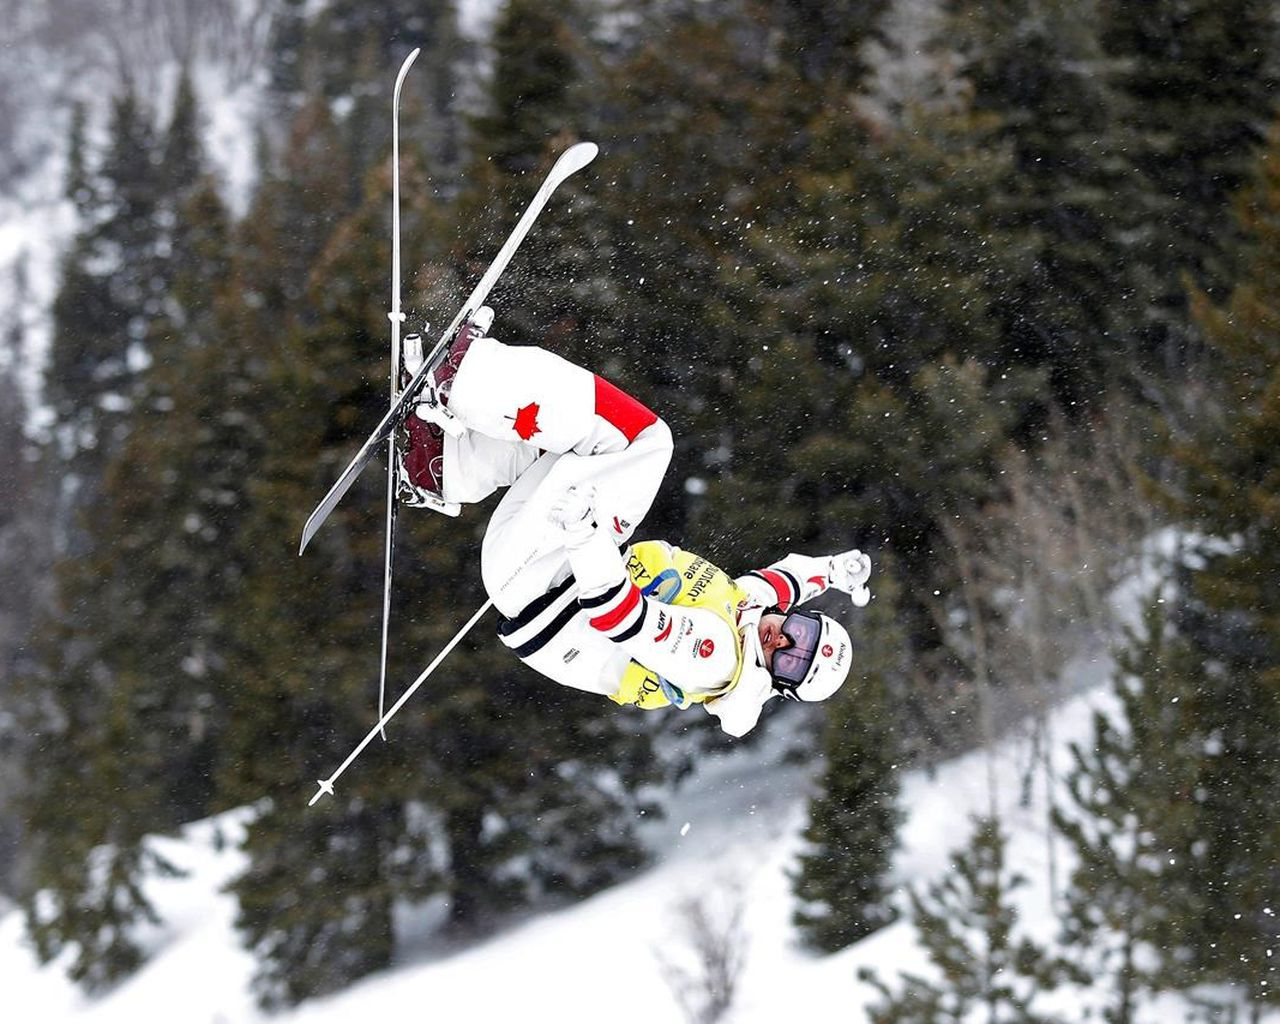
\includegraphics[scale=0.5]{kingsbury.jpg} \\
              Mikaël Kingsbury
            }
            \only<2>{
              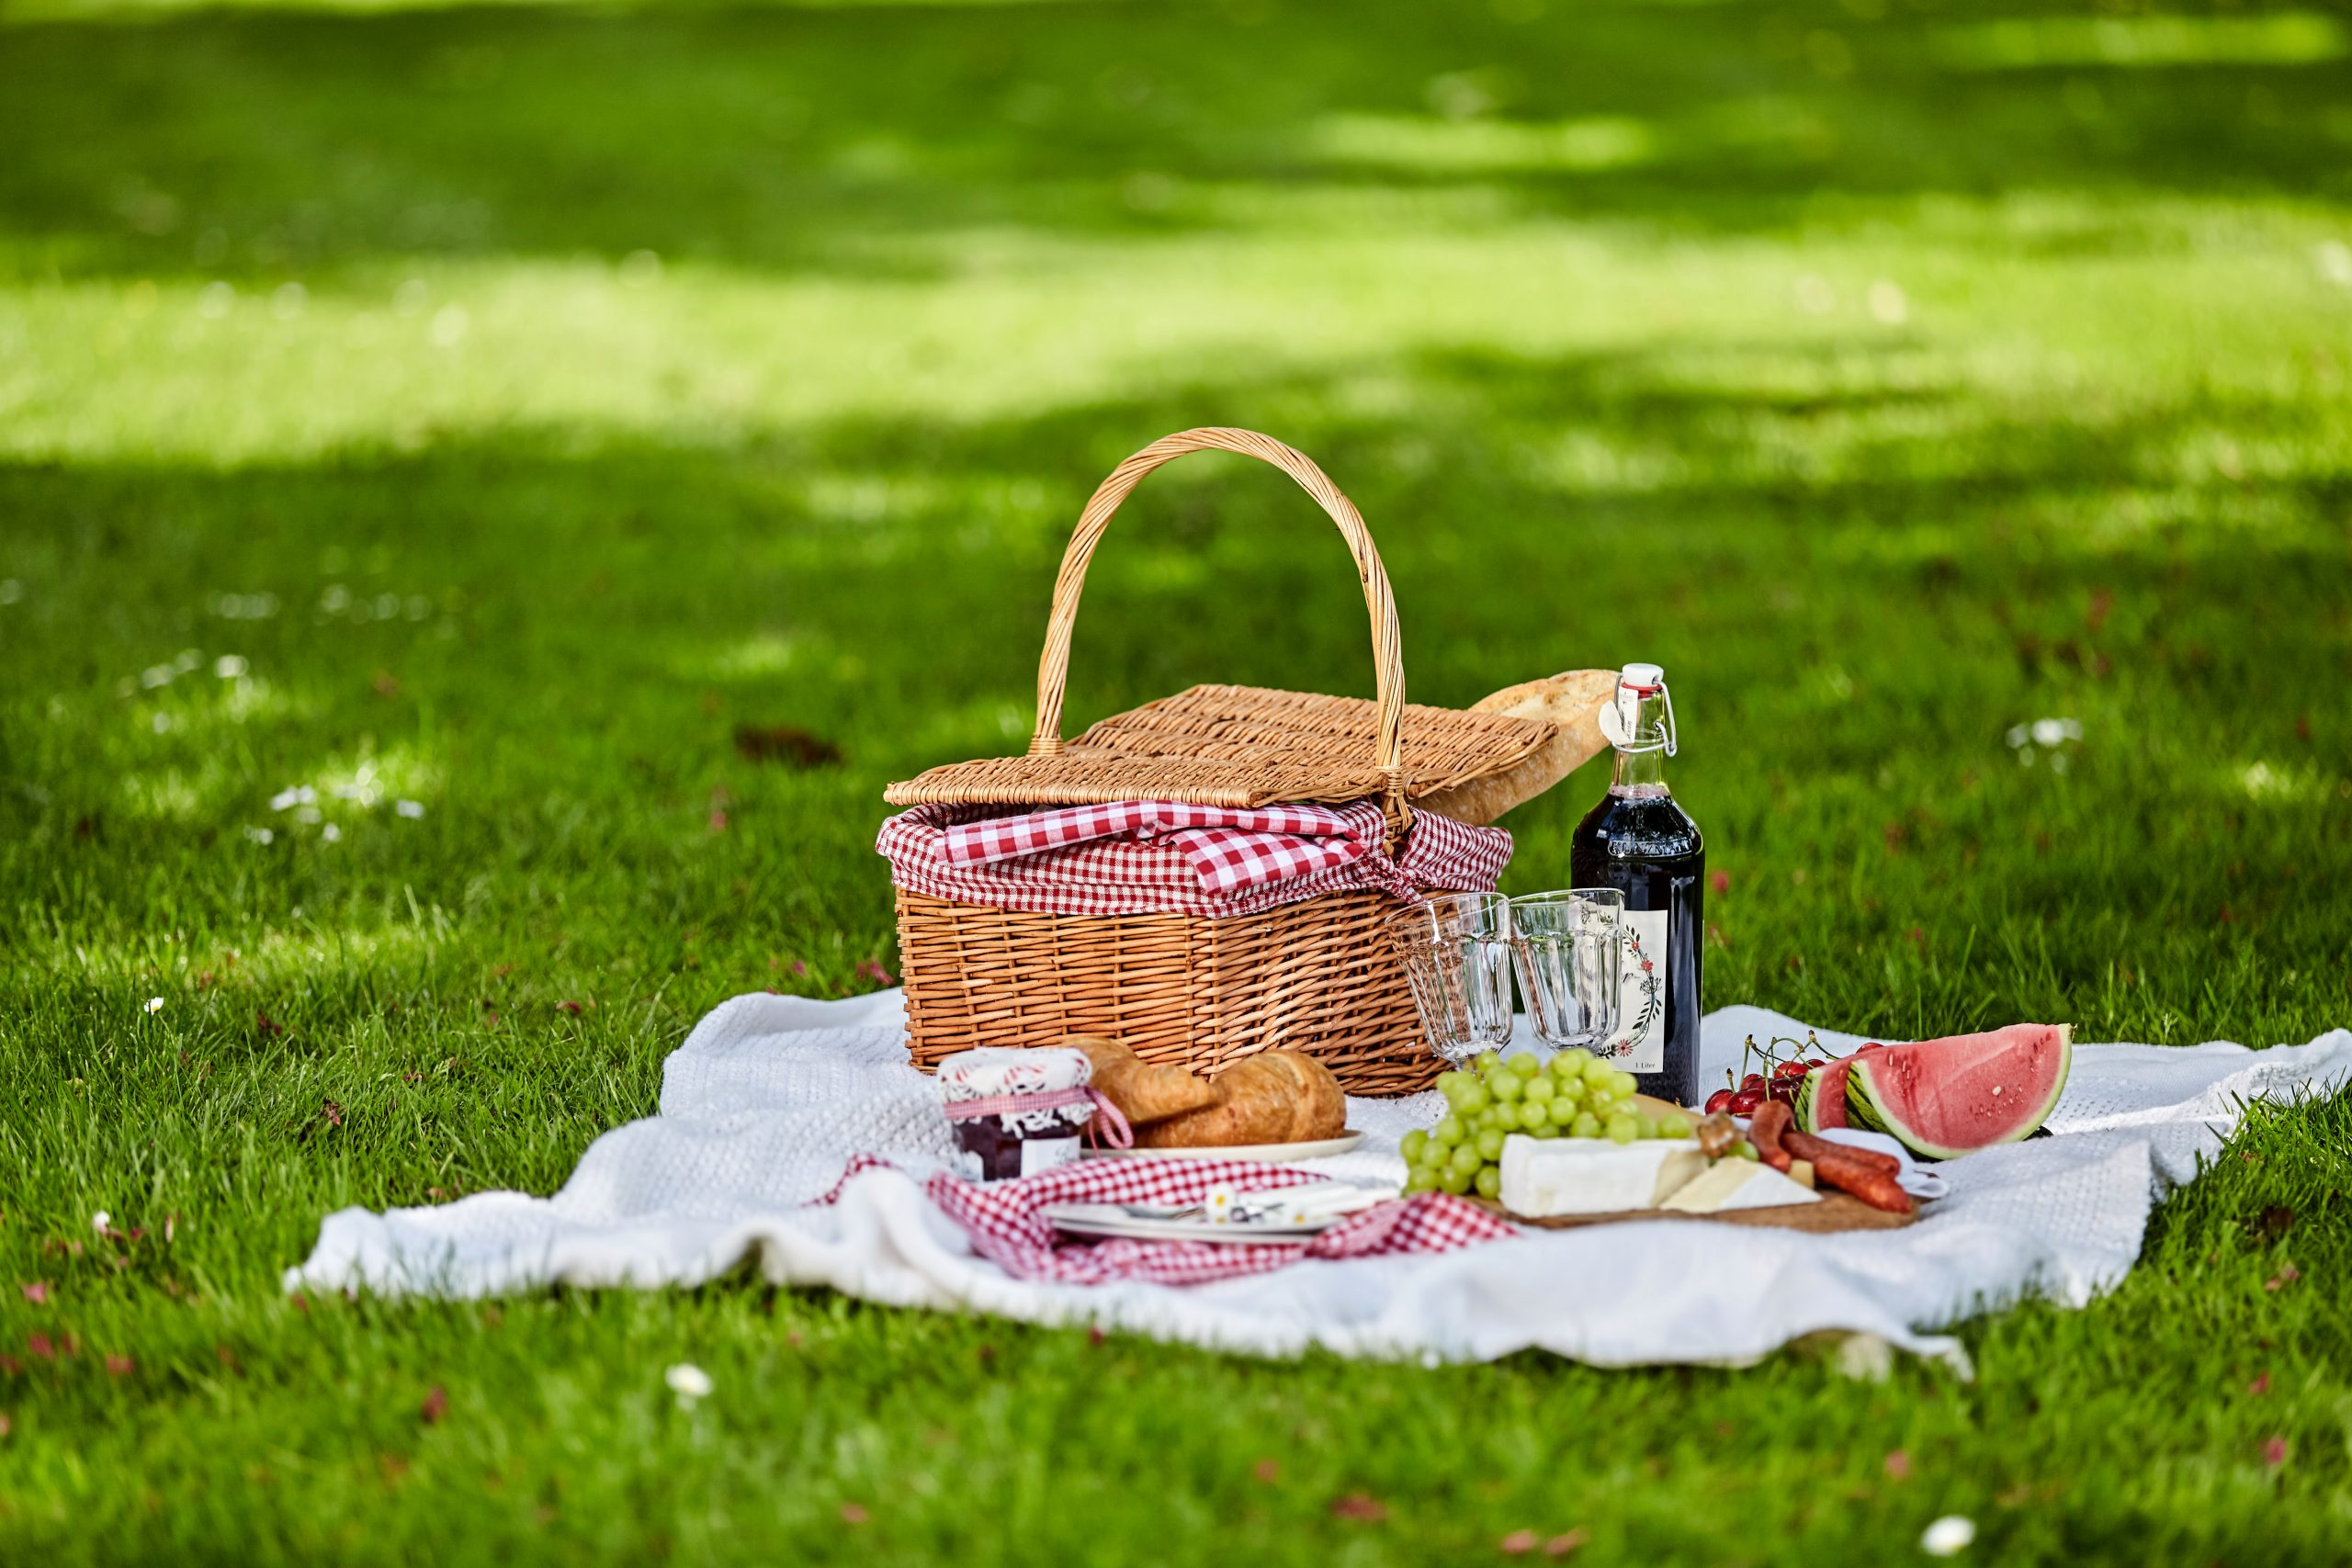
\includegraphics[scale=0.5]{pique-nique.jpeg}
            }
            \only<3>{
              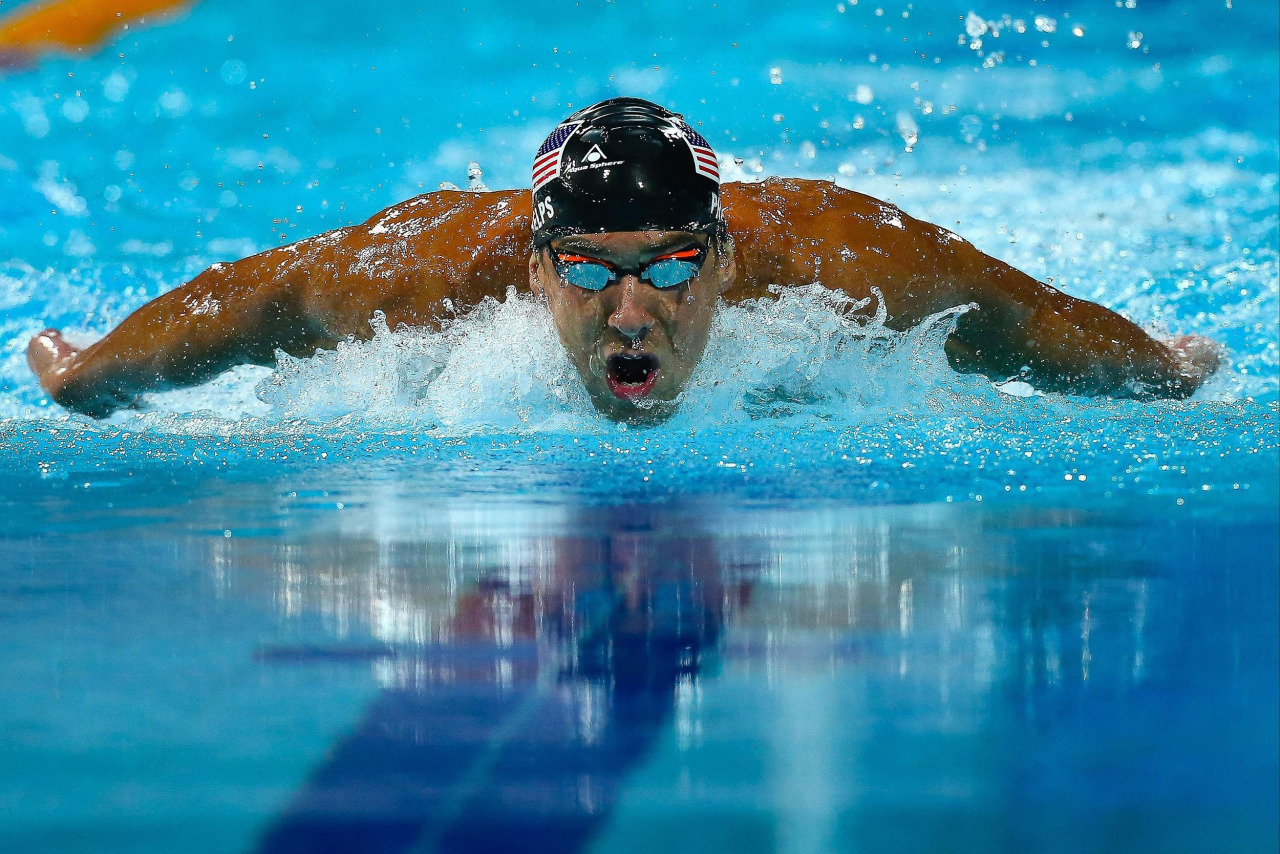
\includegraphics[scale=0.5]{michael_phelps.jpg}
            }
            \only<4>{
              
\includegraphics[scale=0.5]{promenade.jpg}
            }
            \only<5>{
              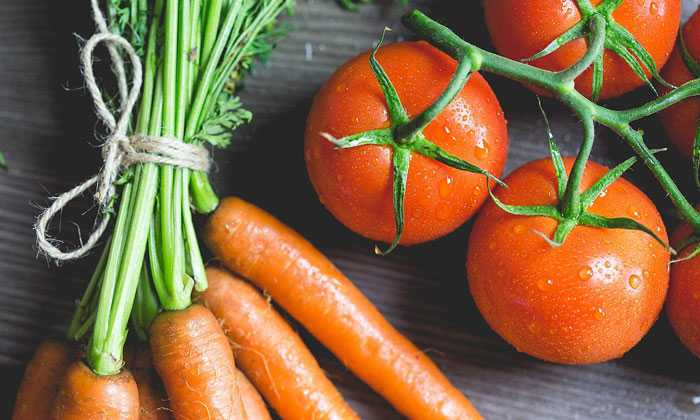
\includegraphics[scale=0.5]{tomates_carrotes.jpg}
            }
            \only<6>{
              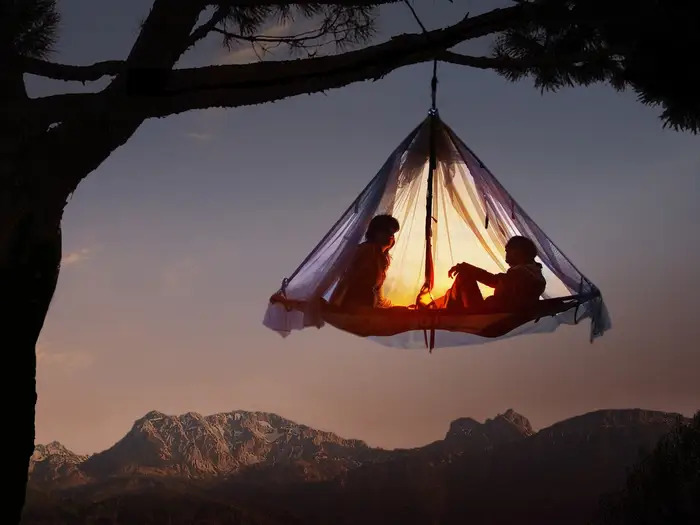
\includegraphics[scale=0.5]{camping.jpg}
            }
            \only<7>{
              
\includegraphics[scale=0.5]{bateau.jpg}
            }
          \end{center}
        \end{minipage}
    \end{columns}
  \end{frame}

  \begin{frame}{}
    \begin{center}
      \Large Quiz
    \end{center}
  \end{frame}

  \begin{frame}{Es-tu plutôt... ?}
    Avec un/e partenaire, discutez vos préférences entre les deux options et pourquoi.
    \begin{description}
      \item[\textbf{Modèle:}] \textit{Es-tu plutôt ville ou campagne?}
      \item[E1:] Je préfère habiter dans une ville. Il y a beaucoup de bons restaurants.
      \item[E2:] Moi, je n'aime pas toutes les voitures. Je préfère le calm de la campagne.
    \end{description}
  \end{frame}

  \begin{frame}{}
    \begin{center}
      \Large Questions?
    \end{center}
  \end{frame}
\end{document}
